\documentclass{article}
\usepackage[utf8]{inputenc}
\usepackage[norsk]{babel}
\usepackage{mathtools} 
\usepackage{hyperref}
\usepackage{listings} 
\usepackage{graphicx}


\begin{document}
\begin{titlepage}
\begin{center}

\vspace*{3cm}
\textsc{\Huge MMI - D3}\\[0.7cm]
\textsc{\medium TTM4100 - Communication Services and Networks}\\[0.3cm]
\textsc{\medium TDT4140 - Software Enigneering}\\[0.3cm]
\textsc{\medium TDT4145 - Data Modeling, Databases and Database Management Systems}\\[0.3cm]
\textsc{\medium TDT4180 - Human-Computer Interaction}\\[0.3cm]

\textbf{\Large Gruppe 7:} \\[0.2cm]
\text{\Large Espen Albert, Finn Inderhaug, Kristoffer Andreas Dalby} \\
\text{\Large Christoffer B. NysÊter, Andreas Wien, Jonas André Dalseth}\\[1cm]

\today

\end{center}
\end{titlepage}
\section{Introduksjon}
Denne rapporten omhandler skjermdesignet og konstruksjonen av brukergrensesnittet til gruppe 7 i fellesprosjektet. Vi skal beskrive vår konseptuelle modell, ta for oss skjermdesignet og gi en konstruksjonsbeskrivelse. 

\section{Konseptuell modell}
%Dere skal her beskrive de begrepene brukeren skal forholde seg til i applikasjonen. Bruk UML for å beskrive klassene, datafeltene i klassene, arv, og relasjoner.



\section{Skjermdesign}

\begin{figure}[h!] 
    \begin{center} 
        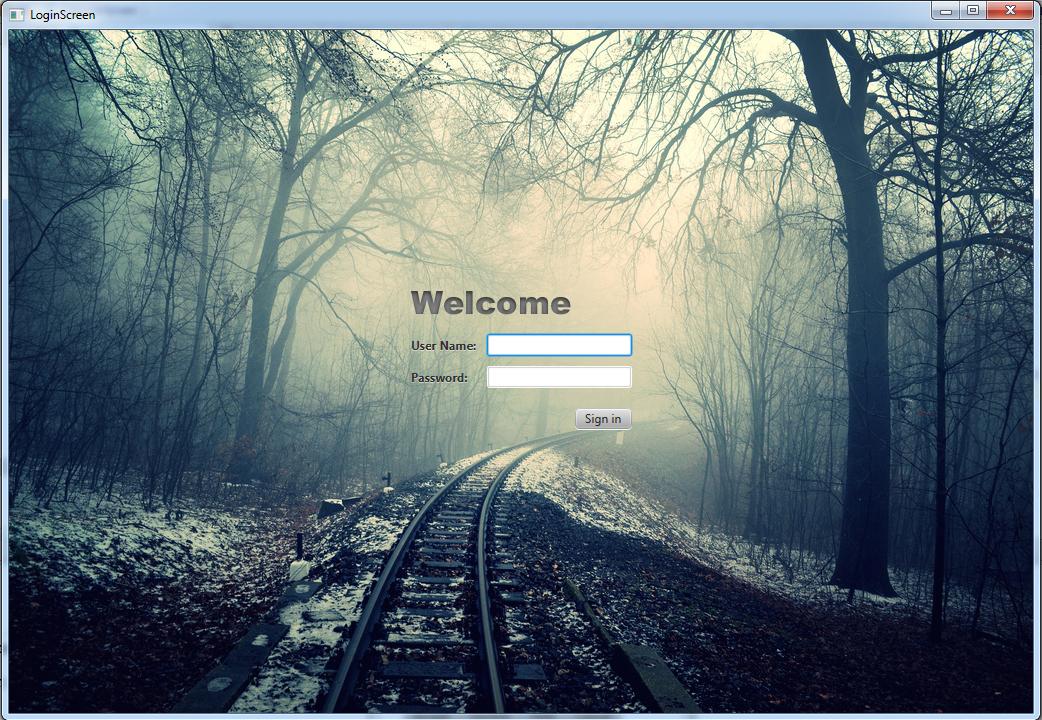
\includegraphics[width=8cm]{LoginScreen.png}
        \caption{Log in screen}
    \label{login}
    \end{center}
\end{figure}

Det første vinduet som møter brukeren er login vinduet. Fra dette vinduet kan brukeren skrive inn brukernavn og passord i de respektive username og password-feltene. Info fra disse feltene lagres som felter i en instans av userklassen. For å logge inn, må brukeren trykke på sign in knappen. Det sjekkes da om brukernavn eksisterer i databasen og om passord evt er riktig. Stemmer disse dataene, åpnes kalendervinduet.


\newpage

\begin{figure}[h!] 
    \begin{center} 
        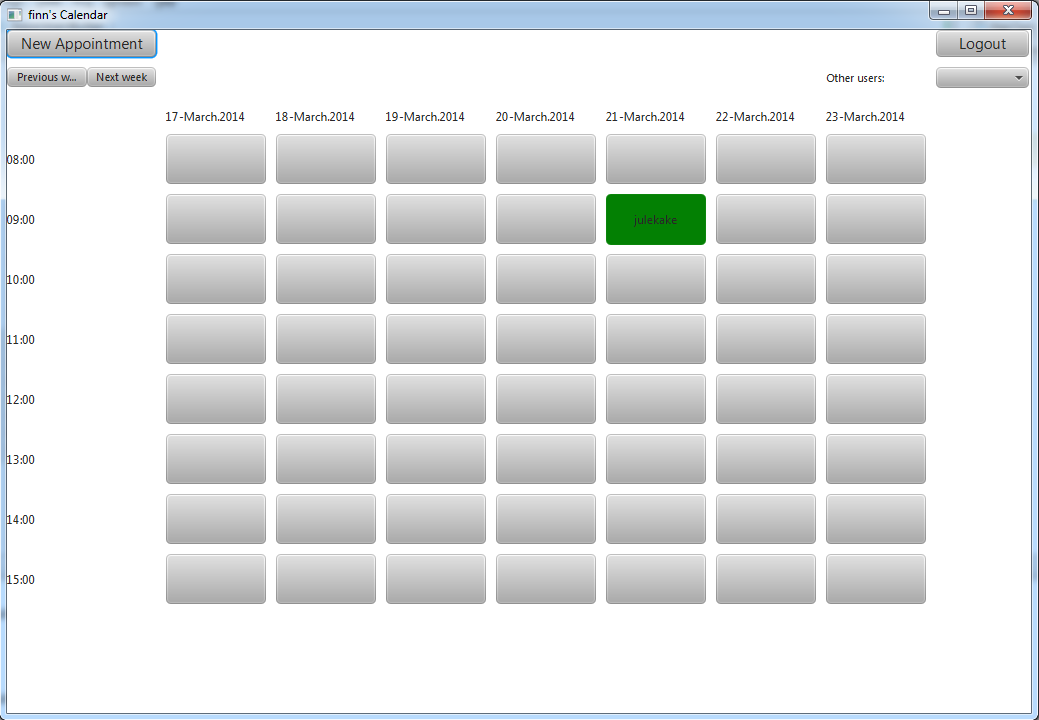
\includegraphics[width=8cm]{MainView.png}
        \caption{Calendar view}
    \label{mainview}
    \end{center}
\end{figure}
I kalendervinduet er det knapper på toppen, hvor det er mulighet til å opprette ny kalender og bla frem og tilbake en uke. I tillegg er det en dropdown meny oppe til høyre hvor du ved å trykke på andres brukernavn kan vise andre brukeres kalender.

Hovedblikkfanget er dog ukeviewet, som er en grid med knapper. Her kan brukeren trykke på knappene for å opprette en avtale i det gitte tidspunktet. Brukeren får da opp et editscreen hvor det er mulig å legge inn data for å opprette en avtale. Om brukeren trykker på en eksisterende avtale får brukeren opp edit-screen hvor brukeren kan endre avtalen. Hvis ikke popper det opp et view-screen hvor brukeren kan vise avtalen.

\newpage

\begin{figure}[h!] 
    \begin{center} 
        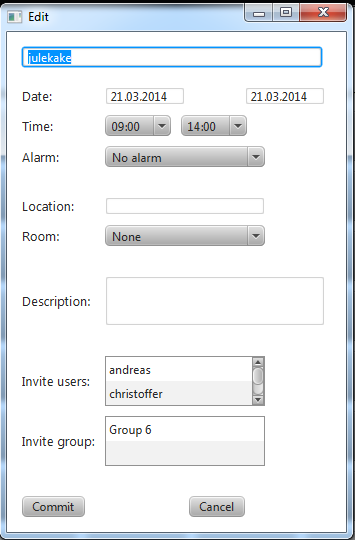
\includegraphics[width=8cm]{EditScreen.png}
        \caption{Edit screen}
    \label{edit}
    \end{center}
\end{figure}
I edtiscreenen er det øverste elementet et tekstfelt hvor brukeren fyller inn navn på avtalen. Deretter er det to tekstfelt for utfylling av dato. Brukeren må fylle inn dato på riktig format, altså :dd.mm.yyyy. Videre er det dropdownmenyer for klokkeslett til elelr fra, og sette tidspunkt for alarmen. I locationtekstfeltet kan brukeren skrive inn hvor avtalen skal foregå. I roomdropdownmenyen får brukeren opp møterom som er ledige i det gitte tidsintervallet avtalen er satt. I description-tekstfeltet kan brukeren legge inn en beskrivelse for arrangementet. I invite users/group-feltene kan man markere de brukerne/gruppene som skal inviteres. Ved å trykke commit-knappen  lagres all informasjonen i et appointmentobjekt og sendes til databasen.

\newpage

\begin{figure}[h!] 
    \begin{center} 
        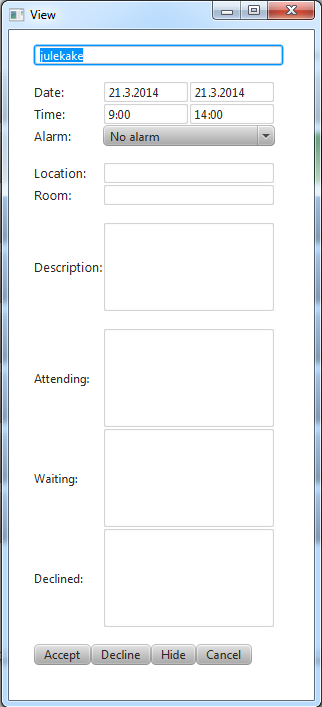
\includegraphics[width=8cm]{ViewScreen.png}
        \caption{Log in screen}
    \label{login}
    \end{center}
\end{figure}
View-screenet inneholder tekstfelt for navn på avtalen, fra og til dato, fra og til klokkeslett, sted, møterom, beskrivelse av arrangementet, hvem som har sagt at de kan komme, hvem som ikke har svart og hvem som ikke kan. I tillegg har vi en dropdownmeny hvor man kan velge når kalenderen skal minne deg på møtet.

\begin{figure}[h!] 
    \begin{center} 
        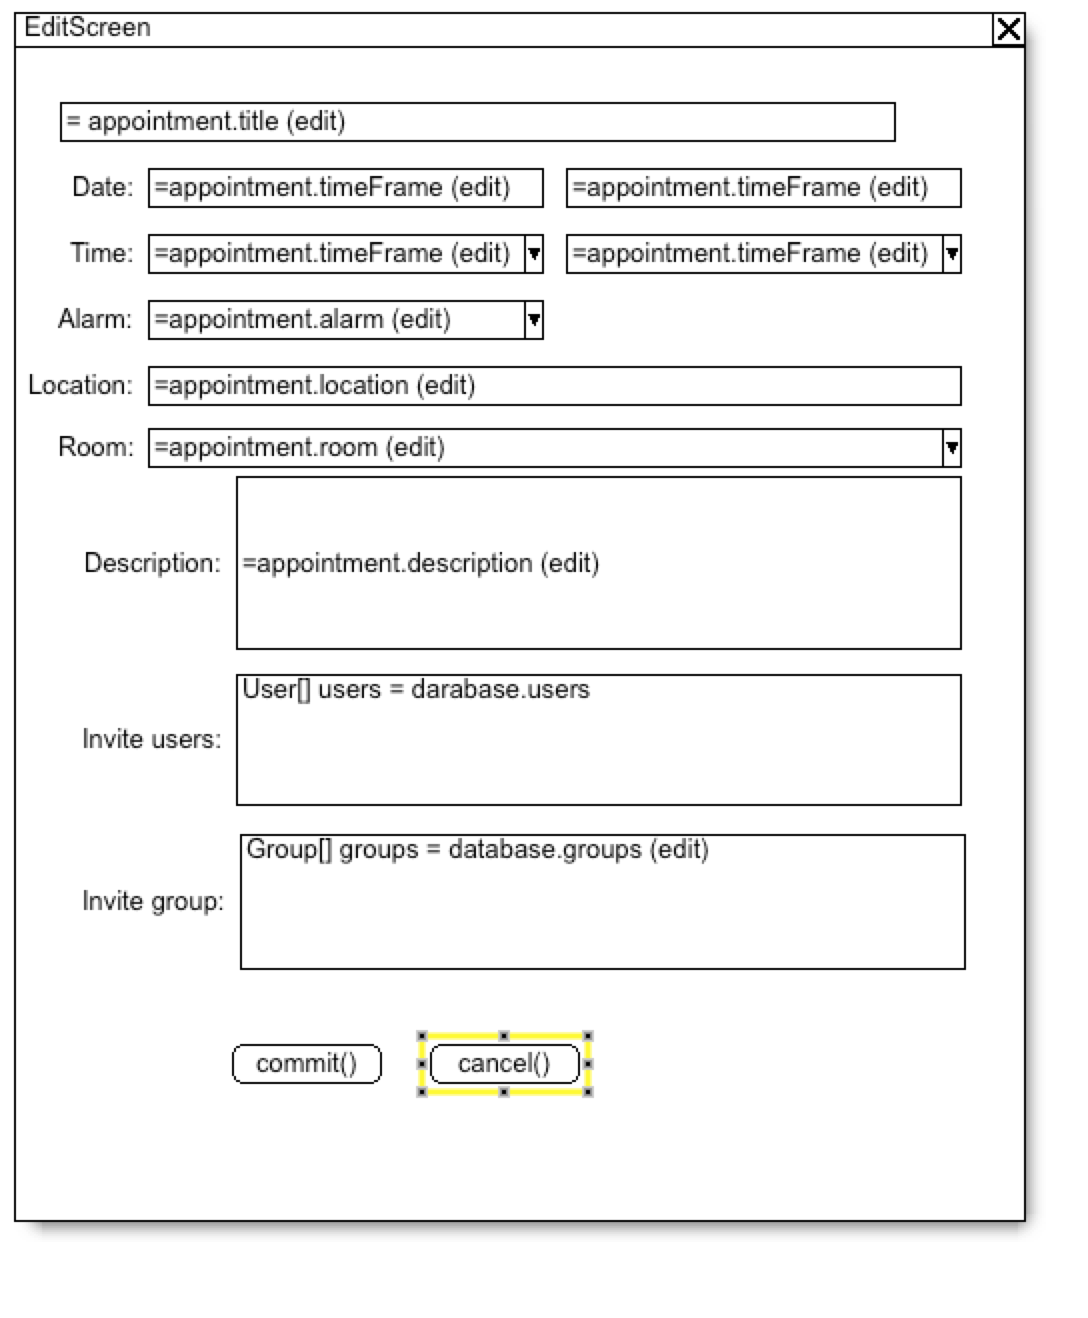
\includegraphics[width=8cm]{editscreendesign.png}
        \caption{Editscreen mockup}
    \label{editmockup}
    \end{center}
\end{figure}

\begin{figure}[h!] 
    \begin{center} 
        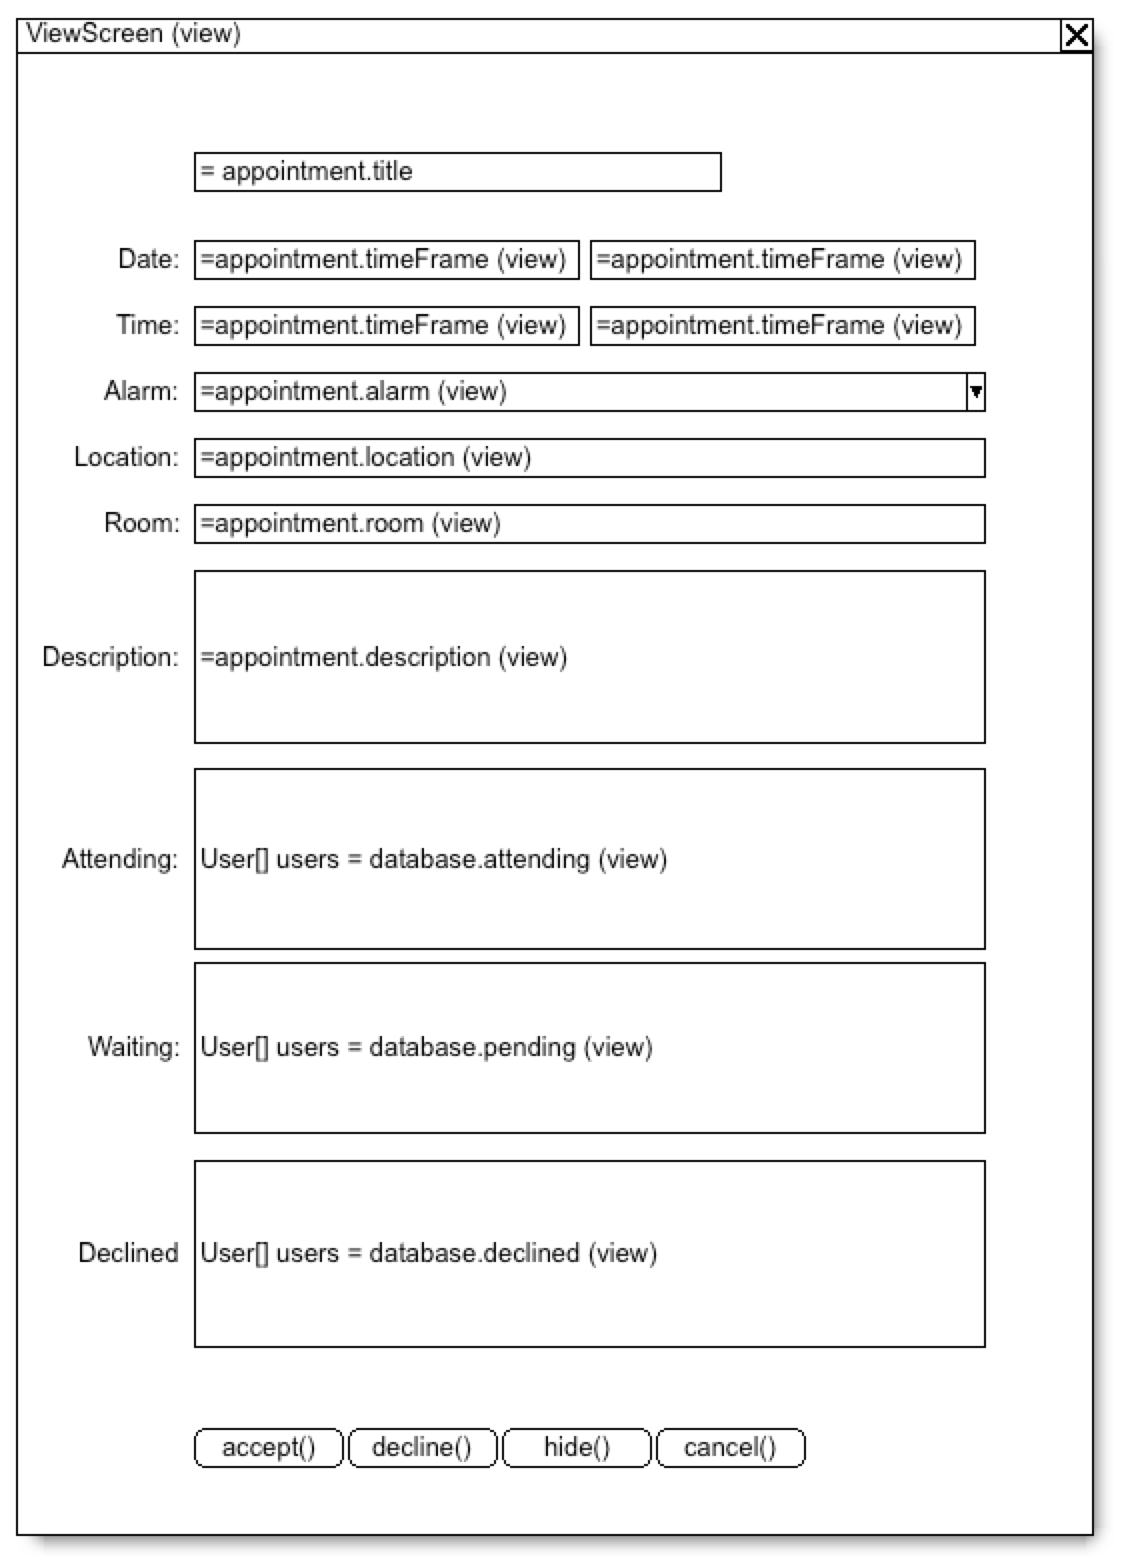
\includegraphics[width=8cm]{viewscreendesign.png}
        \caption{ViewScree mockup}
    \label{viewmockup}
    \end{center}
\end{figure}

\begin{figure}[h!] 
    \begin{center} 
        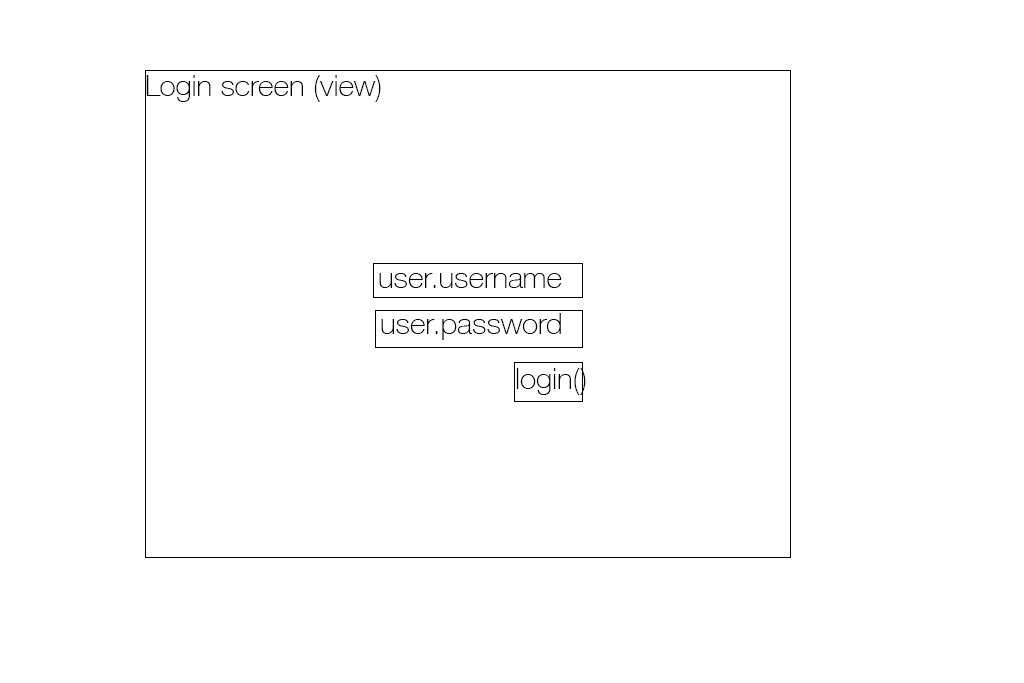
\includegraphics[width=8cm]{login_screen.png}
        \caption{Log in mockup}
    \label{loginmockup}
    \end{center}
\end{figure}

\begin{figure}[h!] 
    \begin{center} 
        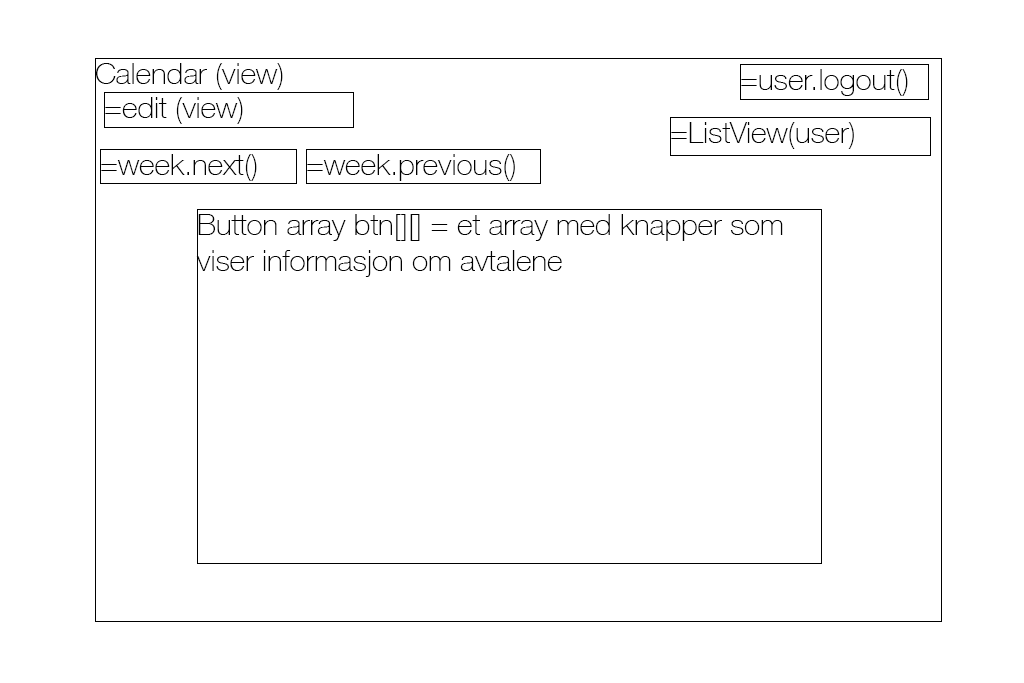
\includegraphics[width=8cm]{Calendar_view.png}
        \caption{Calendar mockup}
    \label{mainmockup}
    \end{center}
\end{figure}





%Dere skal her ta utgangspunkt i kravspesifikasjonen og scenariene fra øving D2. I innleveringen skal dere beskrive grafisk struktur og utforming, kobling mot konseptuell modell, og hvordan alle deler av applikasjonen reagerer på relevante hendelser, som museklikk og tastetrykk. Målet er å spesifisere brukeropplevelsen, dvs. hva brukeren til enhver tid ser og kan gjøre.




\section{Konstruksjonsbeskrivelse}
Oppbygningen er vist i \ref{uikonstruksjon}, og \ref{konstruksjond3} der vi har vist klassene som danner uiet i forhold til hverandre. ComboBoxer og knapper for de ulike viewene er gruppert sammen for bedre leselighet. 

\begin{figure}[h!] 
    \begin{center}  
    	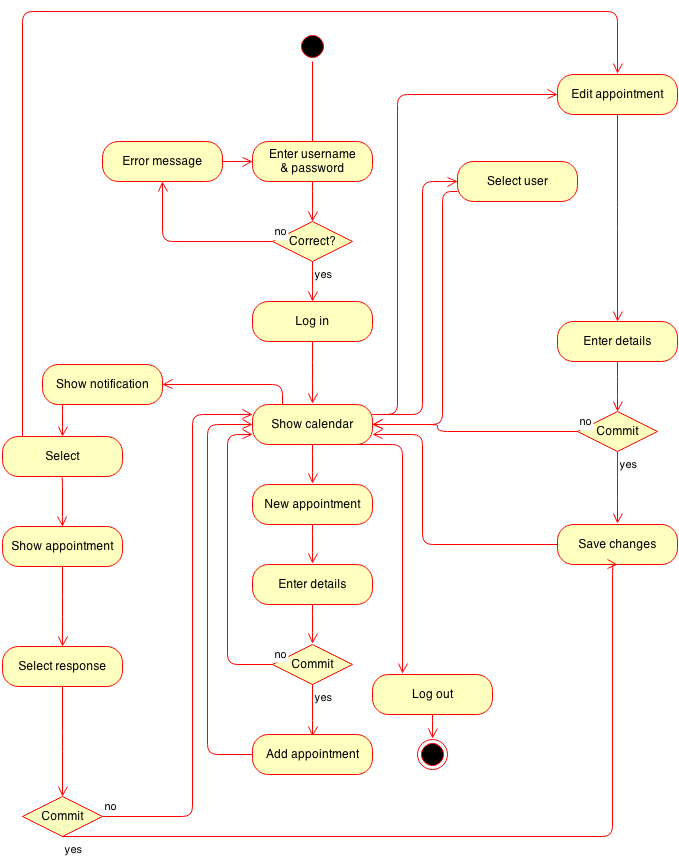
\includegraphics[width=8cm]{calendarStateDiagram.png}
		\caption{Konstruksjon av UI}
	\label{uikonstruksjon}
	\end{center}
\end{figure}


\begin{figure}[h!] 
    \begin{center}  
    	\includegraphics[width=8cm]{Konstruksjond3.png}
		\caption{Konstruksjon av UI}
	\label{konstruksjond3}
	\end{center}
\end{figure}




\end{document}

